\chapter{Methodology} \label{chap:Methodology}

\section{Software Development Life Cycle (SFLC)}

The methodology selected for this project was a mixture of the
incremental and iterative software development lifecycles. This
is a typical methodology selected for machine learning projects
as the exploratory nature of many machine learning projects
necessitates a management method which allows for the flexible
changing of approaches throughout the course of the project.

At a high level, the project is managed using an incremental
approach whereby I found promising ideas from my on-going
literature review and personal exploration of the EMG silent
speech dataset.

Then when I found an approach which I believed was promising,
I conducted initial small-scale experiments to either validate
or disprove my initial assumption, and then scaled up my experiments
iteratively to verify whether or not my hypothesis was valid.

The evaluation metric for each incremental approach was selected
based on the common evaluation metric for that task as reported
in the literature.

\section{Research Plan}

The research plan for my project is orignally based on my
Project Intiation Document (PID), but was modified as the 
data acquisition task for this project was cancelled.

The original research plan was based around finding improvements
to silent speech methods by using the Digital Voicing dataset
(\cite{gaddy2020digital}) open-source dataset and using the
data acquired from myself and participants. Unfortunately due
to financial constraints on the project and the difficulty in
acquiring the EMG data acquisition device which was originally
proposed in the PID, this objective of the project was no
longer achievable. The original project plan was segmented
based along two of the stated objectives of this project,
create an improved model / method for silent speech and data
acquisition.

\begin{center}
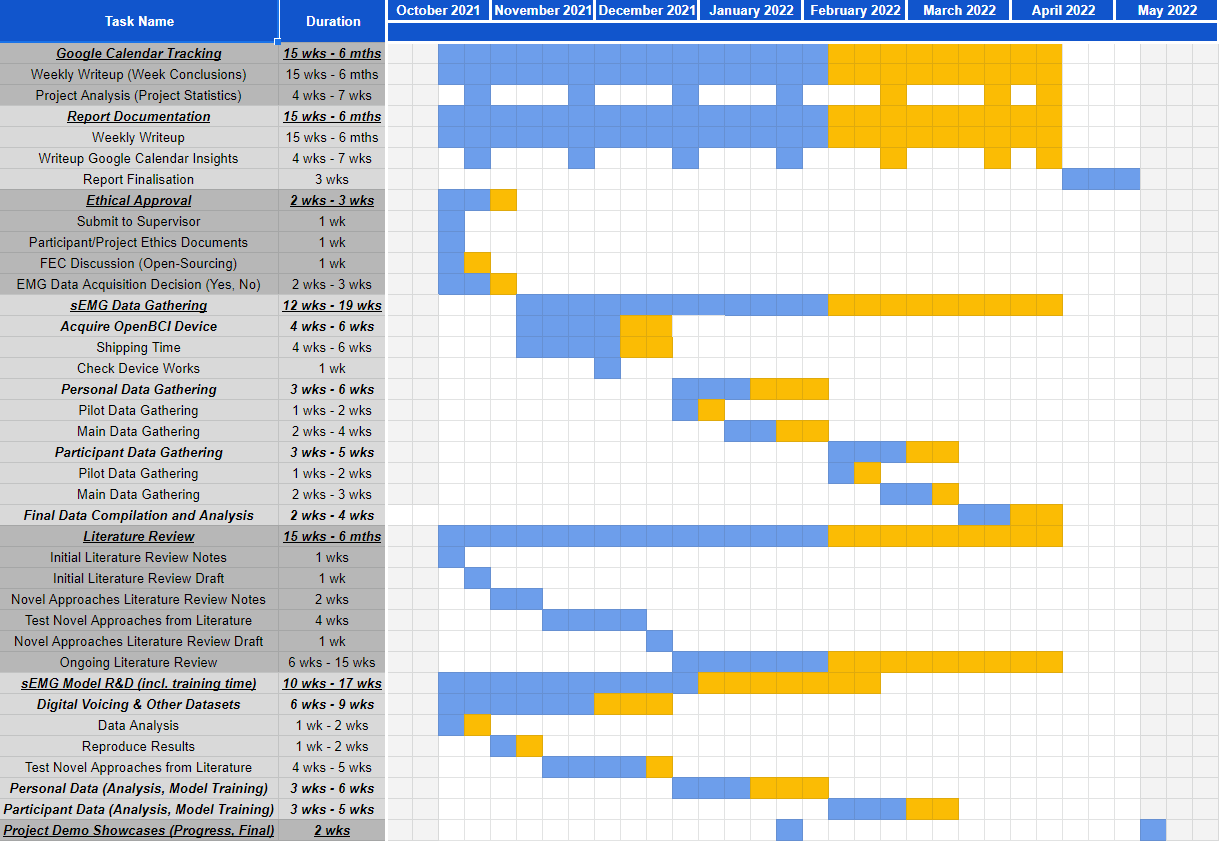
\includegraphics[scale=0.3]{graphics/planning/original_plan.png}
\end{center}

As I only decided to not pursue one of these objectives and
the main objective of my project was still attainable, I
simply stuck to the original project plan and allocated more
time to the research and development for silent speech
methods. However, in-between the first approach and the
second approach of my research, I conducted smaller scale
experiments which have not been mentioned in this report
for brevity.

They are included in the full time line in
the appendix but they are more sporadic and less structured
than the two main approaches explored.

\section{Project Milestones}

This section contains a table which lists the major milestones which were
achieved during this project to give an overview of what was achieved, when it was
achieved and how well the project was managed.

For context, OTR Approach in the table below refers to off the record experiments.
Not every experiment or approach attempt was recorded in this report due to the
number of approaches which did not work, but they are included in the project
milestone table to provide context for how the final documented approaches
were arrived at.

{\small\begin{center}
    \captionof{table}{List of Project Milestones with Dates}
    \begin{tabularx}{\textwidth}{ l l l }
        Date & Type & Milestone \\
        \hline
        19/10/2021 & Admin & PID Submission \\
        October 2021 & Lit Review & General silent speech background \\
        November 2021 & Exploration & Explored EMG Dataset for Interesting Patterns \\
        November 2021 & Approach & Discovered EMG Augmentation \\
        November 2021 & Synth Experiment & Initial Bi-LSTM Model Experiment \\
        December 2021 & Create & Created the EMG synthesis private repo on GitHub \\
        December 2021 & Synth Experiment & Experimented with PyTorch AMP training \\
        December 2021 & Synth Experiment & Experimented with learning rate decay \\
        December 2021 & Synth Experiment & Speech generation \\
        December 2021 & Admin & Email supervisor with status update \\
        December 2021 & Synth Experiment & Switched vocoder to WaveGlow \\
        January 2022 & Admin & Email supervisor with status update \\
        March 2022 & Approach & Considered silent speech recognition \\
        March 2022 & Lit Review & Researched typical speech recognition models \\
        March 2022 & Lit Review & Researched deepspeech2 and conformer models \\
        March 2022 & Lit Review & Researched CTC loss function and decoder \\
        March 2022 & OTR Approach & Researched ASR on direct EMG signals \\
        05/05/2022 & Publish & Switch EMG synthesis repo to GitHub publicly \\
        05/05/2022 & Publish & Released silent speech ASR on GitHub publicly \\
        05/05/2022 & Admin & Switched project to research on SUMS and new ethics
    \end{tabularx}
\end{center}}

{\small\begin{center}
    \captionof{table}{Off-the-record (OTR Approaches)}
    \begin{tabularx}{\textwidth}{ l l l }
        Approach & Notes \\
        Speech recognition on raw EMG signals &
        This approach proved to be unsuccessful because of the complexity
        of converting the raw EMG signals into a suitable latent representation
        which could then be decoded into text. I tried using the hand crafted
        EMG features from (\cite{gaddy2020digital}) and the 5-layer RNN
        layer from the DeepSpeech2 model from this project but to no avail.
        However, this project did make me realise that perfoming ASR directly
        on the predicted mel spectrograms from the transducer model would be
        a worthy direction for research.
    \end{tabularx}
\end{center}}